\chapter{Skills}\label{chap:skills}

\begin{figure}[H]
\centering
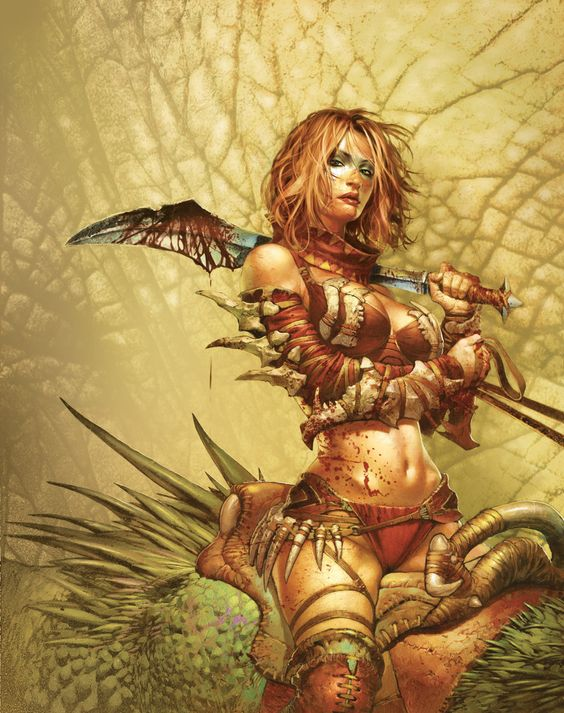
\includegraphics[width=0.6\linewidth]{images/rider.jpg}
\end{figure}

\epigraph{\textit{
    "You can learn much from observing another being. The way the gith hunches before it leaps at you, or how the aarakocra
    circles before it dives. The way the halfling inhales and pauses briefly before shooting his poisoned needles, or how the
    Urikite trader licks his lips before making his final offer. But appearances can deceive. No two creatures are alike.
    Remember that when the gith hunches before casting a defiler spell, or the Urikite trader moistens his lips and spits a
    needle at you." } } { The Oracle, Blue Shrine Scrolls }

\newpage

\section{Complete Skill List}

\begin{table*}[!htb]
\begin{GenesysTable}{Complete Skill List}{complete-skill-list}{ =l +l +X}
Skill                           & Characteristic   & Description\\
\nameref{skill:alchemy}         & Intellect        & Creating and Identifying Potions and Poisons. \\
\nameref{skill:athletics}       & Brawn            & Physical activities such as climbing, running, swimming, etc.\\
\nameref{skill:arcana_attack}   & Intellect        & Identifying and performing Attack magic \\
\nameref{skill:arcana_barrier}  & Intellect        & Identifying and performing Barrier magic \\
\nameref{skill:arcana_dispel}   & Intellect        & Identifying and performing Dispel magic \\
\nameref{skill:arcana_enchantment} & Intellect        & Identifying and performing Enchantment magic \\
\nameref{skill:arcana_illusion} & Intellect        & Identifying and performing Illusion magic \\
\nameref{skill:brawl}           & Brawn            & Unarmed martial arts. \\
\nameref{skill:charm}           & Presence         & Your ability to flatter, whoo and persuation. \\
\nameref{skill:coercion}        & Willpower        & Interrogating, implying and using physical and mental torture. \\
\nameref{skill:cool}            & Presence         & Keeping your nerfe in a variety of situations. \\
\nameref{skill:coordination}    & Agility          & Determines your flexibility and ability to keep your balance. \\
\nameref{skill:crafting}        & Intellect        & Covers your ability to create and repair objects. \\
\nameref{skill:deception}       & Cunning          & Disguising, lying and misleading. \\
\nameref{skill:discipline}      & Willpower        & Represents your mental fortitude to resist threats, coercion and your ability to resist mental attacks. \\
\nameref{skill:education}       & Intellect        & Indicates your literacy, and academic knowledge. \\
\nameref{skill:geography}       & Intellect        & Using maps, following directions and sense of direction. \\
\nameref{skill:leadership}      & Presence         & Rallying troops and allies, convincing crowds of political action. \\
\nameref{skill:medicine}        & Intellect        & Indicates your ability to counteract or administer poisons, identiying and performing medical procedures. \\
\nameref{skill:melee_heavy}     & Brawn            & Using two-handed weapons for physical persuasion. \\
\nameref{skill:melee_light}     & Brawn            & Using one-handed weapons to kill or incapacitate. \\
\nameref{skill:nature}          & Intellect        & Identifying plants and beasts, understanding natural phenomena. \\
\nameref{skill:negotiation}     & Presence         & Haggeling, turning a profit and brokering political agreements. \\
\nameref{skill:perception}      & Cunning          & Your ability to notice threats, clues and conducting surveillance. \\
\nameref{skill:primal_augment}  & Cunning          & Identifying and use Augment spells and effects. \\
\nameref{skill:primal_conjure}  & Cunning          & Identifying and use Conjure spells and effects. \\
\nameref{skill:primal_curse}    & Cunning          & Identifying and use Curse spells and effects. \\
\nameref{skill:primal_shape}    & Cunning          & Identifying and use Shape spells and effects. \\
\nameref{skill:psionics}        & Willpower        & Identifying and using psionic powers. \\
\nameref{skill:ranged}          & Agility          & Using and performance with bows, crossbows, javelins etc. \\
\nameref{skill:resilience}      & Brawn            & Resisting poison, sleep and hostile environments. \\
\nameref{skill:riding}          & Agility          & Using and controlling mounts \\
\nameref{skill:skullduggery}    & Cunning          & Pickpocketing, setting and disabling traps, opening locks and dirty fighting. \\
\nameref{skill:stealth}         & Agility          & Infiltrating, tailing and hiding. \\
\nameref{skill:streetwise}      & Cunning          & Finding and trading black-market goods and tracking in an urban environment. \\
\nameref{skill:survival}        & Cunning          & Locating food and water, handeling animals and tracking in an wilderness setting. \\
\nameref{skill:underworld}      & Intellect        & Locating, understanding and Underworld contacts and methods. \\
\nameref{skill:vigilance}       & Willpower        & Awareness, threat assessment and detecting deception. \\
\end{GenesysTable}
\end{table*}

\section{Special Skill Interactions}
\begin{multicols}{2}

\begin{table*}[!htb]
\begin{GenesysTable}{Social Skill Interaction}{social-skill-interaction}{ =l +X}
Acting Skill         & Opposing Skill \\
Coercion, Leadership & \textbf{Discipline:} The mental fortitude to disobey orders, or the mental strength to resist interrogation and face threats without flinching. \\
Deception            & \textbf{Vigilance:} The mental alertness to notice when someone is lying (since lies and deceptions, by their very nature, are not something someone announces). \\
Charm                & \textbf{Cool:} The ability to keep calm and maintain composure when being charmed or flattered, and to respond politely to flattery without giving away something or giving in to someone’s requests. \\
Negotiation          & \textbf{Negotiation:} Bargaining is usually a back-and-forth between two sides, with both sides using their negotiating skills to try to get as much of what they want as possible. \\
\end{GenesysTable}
\end{table*}

\subsection{Cool vs Vigilance}
Characters should determine their Initiative using the Cool skill when they are aware and ready
for combat (or for whatever situation has resulted in the use of structured gameplay).  For
example, rolling to see who goes first in a quick-draw gunfight or springing an ambush on an
unsuspecting enemy would require Cool, as Cool represents a character’s ability to remain
calm, collected, and focused on the task ahead.

Characters should determine their Initiative using the Vigilance skill when combat (or another
situation resulting in structured gameplay) begins unexpectedly. Two enemies walking around a
corner and running into each other would each use Vigilance to determine Initiative, for example.
Likewise, someone being ambushed would also use Vigilance to determine Initiative (and if they
ended up going earlier in the Initiative order than their ambusher, clearly they were vigilant
enough to spot the ambush at the last second).


\end{multicols}
\section{Skills in Detail}

\subsection{Social Skills}
\begin{multicols}{2}
    \subsubsection{Charm}\label{skill:charm}
\paragraph{You Character should use this skill if ...}
\begin{itemize}
    \item Your character tries to persuade someone to do your character a favor,
      especially if it might be inconvenient, expensive, or even dangerous for that
      person.
    \item Your character tries to appeal to someone's better nature (even if it doesn't
      exist!) to get them to do something out of character for that person.
    \item Your character tries to flirt with, seduce, or make a romantic overture to
      someone.
    \item Your character tries to make themselves look better to everyone around
      them. A lot of politicians and public figures have high ranks in Charm.
    \item Your character performs in front of an audience, acting, playing music,
      telling jokes, or giving a speech.
\end{itemize}
\paragraph{You Character should not use this skill if ...}
\begin{itemize}
    \item Your character is not at all sincere about what they are saying or doing.
      If there’s duplicity or lying involved, your character should use the
      Deception skill.
    \item Your character is being polite, but subtly implying violence or some other
      threat. In those cases, your character should use the Coercion skill.
    \item Your character uses their authority (either through rank, station, or
      natural force of personality) to give orders. These are times for your
      character to use the Leadership skill.
    \item Your character interacts with someone who is already friendly to them,
      or asks someone to do something that is not at all an inconvenience for
      them (generally, you don’t need to use Charm to ask your spouse to pick up
      something from the store on their way home from work).
\end{itemize}

\subsubsection{Coercion}\label{skill:coercion}
\paragraph{You Character should use this skill if ...}
\begin{itemize}
    \item Your character issues a threat, whether or not accompanied by hostile
      actions. Even an implied threat -such as gesturing toward a weapon- falls
      under the Coercion skill.
    \item Your character questions or interrogates a prisoner.
    \item Your character uses physical or psychological torture.
\end{itemize}
\paragraph{You Character should not use this skill if ...}
\begin{itemize}
    \item Your character issues orders backed by the threat of their authority (such
      as threatening troops with courts-martial if they don't follow your character
      into battle). In cases like this, Leadership would be a better skill for
      your character to use.
    \item Your character tries to drive a hard bargain with someone. As long as both
      sides are still getting something out of the deal, Negotiation should be
      the skill to use.
    \item Your character interacts with someone who is already terrified of or
      completely cowed by your character. In these cases, any further threats
      would be superfluous.
\end{itemize}

\subsubsection{Deception}\label{skill:deception}
\paragraph{You Character should use this skill if ...}
\begin{itemize}
    \item Your character tells a lie.
    \item Your character tries to mislead someone through clever wordplay or
      selective omission of certain facts. Your character wears a disguise and
      pretends to be someone else.
    \item Your character wishes to disguise the casting of an Arcane spell.
\end{itemize}
\paragraph{You Character should not use this skill if ...}
\begin{itemize}
    \item Your character actually believes the things they are saying (even if
        they are objectively untrue).
    \item Your character tells a "white lie," a minor falsehood to make someone
        feel better.
\end{itemize}

\subsubsection{Leadership}\label{skill:leadership}
\paragraph{You Character should use this skill if ...}
\begin{itemize}
    \item Your character's allies are suffering from fear, and you want to try to
        rally them.
    \item Your character tries to convince a crowd of citizens to take political
        action.
    \item Your character leads troops into battle and wants to make sure they
        follow your character's orders.
    \item Your character tries to convince a mob of rioters to stand down and
        return to their homes.
\end{itemize}
\paragraph{You Character should not use this skill if ...}
\begin{itemize}
    \item Your character threatens to hurt or kill someone if they don't obey.
        This would be a good use of Coercion, instead.
    \item Your character tries to convince someone to do something simply by being
        friendly and appealing.
    \item Your character should use Charm here.
    \item Your character has formal authority and issues routine orders, especially
        outside of combat or other stressful situations. If there is no good reason
        not to obey your character (and your character has the rank or station to
        issue orders), other people are simply going to obey most mundane commands
        automatically.
\end{itemize}

\subsubsection{Negotiation}\label{skill:negotiation}
\paragraph{You Character should use this skill if ...}
\begin{itemize}
    \item Your character tries to purchase goods or services and wants to haggle
        over the price.
    \item Your character tries to sell goods or services and turn a profit. In
        this case, your character needs to use Negotiation to raise the price.
    \item Your character attempts to broker a political agree- ment or treaty
        between two parties.
\end{itemize}
\paragraph{You Character should not use this skill if ...}
\begin{itemize}
    \item Your character isn't offering anything in return for what they want.
        Getting something for nothing is something your character can try to do
        using other social skills, but Negotiation is predicated on the idea of
        an exchange.
    \item Your character tells someone what to do. Negotiation has to be a bargain,
        so at the end of the interactions, the opposing party has agreed to do
        something, not been ordered to do it.
    \item Your character wants to buy something for a previously established
        price.
\end{itemize}

\end{multicols}
\hrulefill
\subsection{General Skills}
\begin{multicols}{2}
\subsubsection{Alchemy}\label{skill:alchemy}
The difficulty of preparing a potion should generally correspond
to its rarity: generally by dividing the rarity by 2 and rounding up.
The resulting number should be the difficulty of the check to brew the
potion. For instance, if your character wants to make a healing poultrice
of rarity 2, the base difficulty of the check is Easy (\difficulty).
If your character doesn’t have the proper equipment or ingredients,
the difficulty may be higher.
\paragraph{You Character should use this skill if ...}
\begin{itemize}
    \item Your character tries to identify a potion by taste.
    \item Your character wants to name the ingredients needed for a certain elixir.
    \item Your character tries to prepare a potion, elixir, poultice, tonic, or
        similar compound with wondrous or magical effects.
    \item Your character attempts to prepare a remedy for a disease or illness.
    \item Your character attempts to prepare a poison.
\end{itemize}
\paragraph{You Character should not use this skill if ...}
\begin{itemize}
    \item Your character attempts to enchant an otherwise mundane liquid.
    \item Your character desires to heal someone directly through medical treatment
        of their wounds.
    \item Your character seeks to transmute lead into gold. That would clearly
        be magic!
\end{itemize}

\subsubsection{Athletics}\label{skill:athletics}
\paragraph{You Character should use this skill if ...}
\begin{itemize}
    \item Your character attempts to climb up or down a structure, particularly
        when the climb may be tricky or the drop to the bottom is significant.
    \item Your character tries to jump, either vertically or horizontally. Leaping
        across a deep chasm or trying to jump up and grab a fire escape to get
        away from an angry dog are both situations when your character needs to
        make an Athletics check.
    \item Your character attempts to run for an extended time.
\end{itemize}
\paragraph{You Character should not use this skill if ...}
\begin{itemize}
    \item Your character attempts an activity without any chances of failure. If
        your character goes for an early morning jog, or jumps over a small log,
        they don't need to bother making a check.
    \item Your character attempts a physical activity that relies more on hand-eye
        coordination and general agility than straight strength. Engaging in
        parkour and freerunning, swinging on a rope and rappelling down a surface,
        and most forms of gymnastics are activities better represented by the
        Coordination skill.
\end{itemize}

\subsubsection{Cool}\label{skill:cool}
\paragraph{You Character should use this skill if ...}
\begin{itemize}
    \item Your character begins laying a trap, staging an ambush, or otherwise
        setting up a combat encounter in which your character initiates the
        combat and has to judge the right time to do so.
    \item Your character needs to stay calm and unaffected when being flattered
        or charmed by someone.
    \item Your character needs to refrain from saying or doing something foolish
        during a tense situation.
    \item Your character needs to keep their nerve in a tense situation, such as
        when charging an Erdlu into a spear wall.
    \item Your character plays a card game or other game of chance in which bluffing,
        luck, and gambling are all intertwined.
\end{itemize}
\paragraph{You Character should not use this skill if ...}
\begin{itemize}
    \item Your character tries to prevent being surprised. The Vigilance skill
        would work better in that situation.
    \item Your character tries to maintain inner self-control, such as when
        meditating or resisting the effects of fear. When your character is
        concerned with inner composure, they should use the Discipline skill.
\end{itemize}

\subsubsection{Coordination}\label{skill:coordination}
\paragraph{You Character should use this skill if ...}
\begin{itemize}
    \item Your character tries to swing back and forth on a rope or rappel down
        a structure.
    \item Your character walks across a narrow surface while trying to keep their
        balance.
    \item Your character tries to squeeze into a tiny or cramped space such as a
        crawlspace, sewer pipe, air duct, or narrow crevice.
    \item Your character falls and needs to try to slow the fall or land safely.
    \item Your character needs to escape from physical restraints (such as
        handcuffs or ropes) and wants to contort their limbs or hands so that they
        can slip out of their bindings.
\end{itemize}
\paragraph{You Character should not use this skill if ...}
\begin{itemize}
    \item Your character tries to climb up or down a rope or climb up a structure.
        This activity relies more on strength than agility, and calls for an
        Athletics check instead.
    \item Your character falls from a short height or onto something soft enough
        that they won't suffer damage when they land, or is in any similar
        situation that has no consequences for failure (is lowered down a structure
        in a firmly secured harness, for example).
\end{itemize}

\subsubsection{Crafting}\label{skill:crafting}
\paragraph{You Character should use this skill if ...}
\begin{itemize}
    \item Your character needs to repair a damaged weapon, cart, or other piece
        of equipment.
    \item Your character needs to identify any parts or tools necessary prior to
        completing a job. This can save time and money on the project.
    \item Your character has access to a supply of components and tools and wants
        to design a completely new device.
    \item Your character needs to sabotage an enemy's caravan cart or find a weak
        point in their defenses.
    \item Your character needs to build an item or modify it.
\end{itemize}
\paragraph{You Character should not use this skill if ...}
\begin{itemize}
    \item Your character has just a simple task like hanging a door, or fixing a
        shoe.
\end{itemize}

\subsubsection{Discipline}\label{skill:discipline}
\paragraph{You Character should use this skill if ...}
\begin{itemize}
    \item Your character confronts something terrifying and wants to avoid fleeing
        in horror (or to avoid other debilitating effects of fear).
    \item Your character tries to keep their sanity in the face of something that
        defies reality and rational thought.
    \item Your character wants to heal strain they are suffering from at the end
        of an encounter.
    \item Your character wants to meditate, calm their mind, and reach a mental
        equilibrium.
\end{itemize}
\paragraph{You Character should not use this skill if ...}
\begin{itemize}
    \item Your character tries to keep their composure in a social setting and
        avoid letting their emotions show.
    \item Your character would make a Cool check instead.
    \item Your character catches a lie as it is being told. Notic- ing a lie
        depends on your character’s Vigilance.
\end{itemize}

\subsubsection{Medicine}\label{skill:medicine}
\begin{table*}[!htb]
\begin{GenesysTable}{Medicine Check Difficulty}{medicine-check-difficulty}{ =X +X}
State of Health                                        & Difficulty \\
Current wounds equal half of wounds threshold or less  & \textbf{Easy:} (\difficulty) \\
Current wounds equal more than half of wound threshold & \textbf{Average:} (\difficulty\difficulty) \\
Current wounds exceed wound threshold                  & \textbf{Hard:}  (\difficulty\difficulty\difficulty) \\
Criticl Injury                                         & Critical Injury severity Rating \\
\end{GenesysTable}
\end{table*}
\paragraph{You Character should use this skill if ...}
\begin{itemize}
    \item They or another character has suffered wounds, and your character wants
        to heal those wounds.
    \item Your character tries to counteract or administer a poison.
    \item Your character needs to cure a disease.
    \item Your character creates a new pharmaceutical (or recreational) drug.
    \item They or another character has suffered a Critical Injury, and your
        character wants to heal it.
    \item Your character performs a complex medical procedure such as surgery.
\end{itemize}
\paragraph{You Character should not use this skill if ...}
\begin{itemize}
    \item Your character researches a disease or poison. While studying a disease
        or poison directly might require Medicine, the act of researching requires
        an Education check.
    \item Your character tries to heal their own strain at the end of an encounter.
        Recovering from strain at the end of an encounter requires Discipline or Cool.
    \item Your character tries to administer poison through slight of hand, such
        as by dropping it in a drinking cup or surreptitiously injecting it into
        an unsuspecting target. The inherent subterfuge in this activity makes
        that a Skulduggery check.
\end{itemize}

\subsubsection{Perception}\label{skill:perception}
\paragraph{You Character should use this skill if ...}
\begin{itemize}
    \item Your character wants to search a crime scene for clues.
    \item Your character wants to study the surrounding landscape for possible
        threats.
    \item Your character conducts surveillance on an unaware target from a
        distance.
    \item Your character studies an ancient relic, trying to spot any minute details
        that could reveal its purpose or construction.
\end{itemize}
\paragraph{You Character should not use this skill if ...}
\begin{itemize}
    \item Your character tries to avoid being surprised during an ambush. Constant,
        unconscious awareness of your character's surroundings is a function of
        the Vigilance skill.
    \item Your character is being lied to, and you're trying to find out if your
        character noticed or not. Again, Vigilance is the skill for this situation.
    \item Your character tries to follow a trail or track a foe through the
        wilderness. The Survival skill covers these activities.
\end{itemize}

\subsubsection{Resilience}\label{skill:resilience}
\paragraph{You Character should use this skill if ...}
\begin{itemize}
    \item Your character tries to go without sleeping for days on end, and you
        need to see if they stay awake.
    \item Your character ingests a toxin, and you need to see how bad the effects
        are.
    \item Your character endures a hostile environment (somewhere too hot, too
        cold, or even too polluted) for days on end.
    \item Your character attempts to recover from a Critical Injury on their own,
        without medical attention.
\end{itemize}
\paragraph{You Character should not use this skill if ...}
\begin{itemize}
    \item Your character tries to do something that isn't beyond the limits of
        normal endurance. Going for a day-long hike wouldn't call for a Resilience
        check unless the hike is through the Rocky Mountains in a sandstorm.
    \item Your character immediately stops and rests to recover fully at the end
        of the activity. If there's no need to track lasting consequences, there's
        no need to make the check.
\end{itemize}

\subsubsection{Riding}\label{skill:riding}
\paragraph{You Character should use this skill if ...}
\begin{itemize}
    \item Your character flees from pursuers who are also mounted, or fast enough
        to potentially catch up.
    \item Your character tries to joust at a tournament.
    \item Your character competes in a friendly (or not so friendly) race.
    \item Your character tries to catch up to enemies with a significant head
        start.
    \item Your character's mount panics during a storm, and your character needs
        to get the creature under control.
\end{itemize}
\paragraph{You Character should not use this skill if ...}
\begin{itemize}
    \item Your character travels without any immediate danger.
    \item Your character makes an attack from horseback. The additional difficulty
        brought about by attacking from a horse should be factored into the combat
        check's difficulty, generally in the form of one or more \difficulty.
    \item Your character tries to tame a wild animal. In this case, your character
        uses the Survival skill.
\end{itemize}

\subsubsection{Skullduggery}\label{skill:skullduggery}
\paragraph{You Character should use this skill if ...}
\begin{itemize}
    \item Your character attempts to pick someone's pocket or lift their wallet.
    \item Your character tries to pick a lock or disable a trap.
    \item Your character would also use Skulduggery to set a trap in the first
        place.
    \item Your character attempts to distract an opponent through guile or a feint,
        such as by throwing a handful of dirt in their eyes during a fight.
    \item Your character tries to surreptitiously slip a poison into someone's
        food or drink.
\end{itemize}
\paragraph{You Character should not use this skill if ...}
\begin{itemize}
    \item Your character attempts to sneak into a location unnoticed. Your
        character needs to make a Stealth check instead.
    \item Your character attempts to pick someone's pocket when that person is
        helpless or incapacitated. This doesn't require a check at all.
    \item Your character tries to make a poison. Your character needs Alchemy to
        make poisons or toxins, but they do need Skulduggery to use them.
\end{itemize}

\subsubsection{Stealth}\label{skill:stealth}
\paragraph{You Character should use this skill if ...}
\begin{itemize}
    \item Your character attempts to hide from someone.
    \item Your character tries to tail someone through a crowd, and to do it
        without being noticed.
    \item Your character tries to infiltrate a government installation while
        avoiding both electronic security and human guards.
    \item Your character tries to move quietly through a house.
\end{itemize}
\paragraph{You Character should not use this skill if ...}
\begin{itemize}
    \item Your character tries to pick someone's pocket. Your character needs
        Skulduggery for this activity.
    \item Your character tries to remain hidden when their opponent has no chance
        of spotting them, such as if they try to avoid being seen by an flying
        Aarakocra during a blizzard at midnight.
    \item Your character has no realistic chance of hiding from an opponent, such
        as if trying to hide from a nearby person while in the middle of miles of
        salt flats at noon.
\end{itemize}

\subsubsection{Streetwise}\label{skill:streetwise}
\paragraph{You Character should use this skill if ...}
\begin{itemize}
    \item Your character looks for a merchant who sells black-market goods or
        illegal services.
    \item Your character wants to understand particular references or slang in
        a conversation.
    \item Your character tries to approach criminals and start up a conversation
        without appearing like an outsider or a threat.
    \item Your character tries to find their way around an unfamiliar city.
    \item Your character tries to track and hunt someone somewhere in a city.
\end{itemize}
\paragraph{You Character should not use this skill if ...}
\begin{itemize}
    \item Your character tries to find their way around a rural or wilderness
        environment. In this case, your character should be using Survival.
    \item Your character interacts with the upper crust of society. Charm (or
        possibly Deception or Coercion) may serve the character better here.
    \item Your character has already established themself as a member of the
        criminal underworld, and is continuing to interact with other criminals.
        Streetwise lets your character fit in, know how to act, and know what
        topics to bring up and what to avoid. However, it shouldn't replace
        social skills.
\end{itemize}

\subsubsection{Survival}\label{skill:survival}
\paragraph{You Character should use this skill if ...}
\begin{itemize}
    \item Your character is trapped in the wilderness and needs to find food and
        potable water.
    \item Your character needs to notice approaching severe weather and know how
        to prepare for it.
    \item Your character needs to follow a crude map or directions through a rural
        area to find a specific location.
    \item Your character tries to tame or calm a wild animal, or handle a
        domesticated animal.
    \item Your character hunts something (or someone!) through a wilderness
        setting.
\end{itemize}
\paragraph{You Character should not use this skill if ...}
\begin{itemize}
    \item Your character uses a highly accurate and detailed map to find a location.
    \item Your character tries to find their way around an urban environment. In
        this case, your character should be using Streetwise.
    \item Your character interacts with an animal that already likes or respects
        your character, or your character asks an animal to do something completely
        within their nature (they wouldn't need to make a Survival check to get a
        dog to play "fetch," for example).
\end{itemize}

\subsubsection{Vigilance}\label{skill:vigilance}
\paragraph{You Character should use this skill if ...}
\begin{itemize}
    \item Your character just got ambushed, and you are rolling to determine
        Initiative order. A high Vigilance means your character has a better chance
        of reacting quickly to the threat.
    \item Your character is being lied to; the opponent's Deception check is opposed
        by your character's Vigilance skill.
    \item Your character has a chance to notice important details in their
        surroundings while not looking for them directly.
\end{itemize}
\paragraph{You Character should not use this skill if ...}
\begin{itemize}
    \item You are determining Initiative order when your character is not surprised
        (such as when they are the ambushers, instead of the ambushed). In this
        case, your character uses Cool instead.
    \item Your character actively looks for something. This calls for a Perception
        check.
\end{itemize}

\end{multicols}
\hrulefill
\subsection{Combat Skills}
\begin{multicols}{2}
\subsubsection{Brawl}\label{skill:brawl}
\paragraph{You Character should use this skill if ...}
\begin{itemize}
    \item Your character fights with their bare hands or a weapon specifically
        designed to augment an unarmed attack, such as cestus or punchik (or even
        a roll of bits).
    \item Your character tries to pin, grapple, or hold someone.
    \item Your character uses some form of unarmed martial art.
\end{itemize}
\paragraph{You Character should not use this skill if ...}
\begin{itemize}
    \item Your character fights with a projectile weapon or a thrown weapon. If
        your character is targeting someone who is not within arm's reach, they
        should be using the Ranged skill.
    \item Your character tries to fix or modify a melee weapon. Repairing or
        creating weapons is usually handled by the Mechanics skill.
\end{itemize}

\subsubsection{Melee (Heavy)}\label{skill:melee_heavy}
\paragraph{You Character should use this skill if ...}
\begin{itemize}
    \item Your character fights with a long spear, gouge, quarterstaff, two-handed
        club, or other large weapon that requires two hands to wield.
    \item Your character picks up a heavy tree branch and tries to crush someone's
        skull with it.
\end{itemize}
\paragraph{You Character should not use this skill if ...}
\begin{itemize}
    \item Your character fights with a knife, dirk, one-handed club, light spear,
        or other weapon that can be swung easily with one hand.
\end{itemize}

\subsubsection{Melee (Light)}\label{skill:melee_light}
\paragraph{You Character should use this skill if ...}
\begin{itemize}
    \item Your character fights with a knife, dirk, one-handed club, light spear,
        or other weapon that can be swung easily with one hand.
    \item Your character wants to hit someone with their shield.
\end{itemize}
\paragraph{You Character should not use this skill if ...}
\begin{itemize}
    \item Your character fights with a long spear, gouge, quarterstaff, two-handed
        club, or other large weapon that requires two hands to wield.
\end{itemize}

\subsubsection{Ranged}\label{skill:ranged}
\paragraph{You Character should use this skill if ...}
\begin{itemize}
    \item Your character fights with a longbow, blowgun, sling or other ranged weapon.
\end{itemize}
\paragraph{You Character should not use this skill if ...}
\begin{itemize}
    \item Your character fights with any kind of close combat weapon. Those are
        handled by the Melee skill.
    \item Your character uses a ranged weapon to hit someone within arm's reach,
        such as by loading a sling and use it like a club. Even though they're
        using a ranged weapon, they’re using it as if it were a melee weapon, and
        the check should be handled by the Melee skill.
    \item Your character tries to fix or modify a ranged weapon. Repairing or
        creating weapons is usually handled by the Crafting skill.
\end{itemize}

\end{multicols}
\hrulefill
\subsection{Knowledge Skills}
\begin{multicols}{2}
\subsubsection{Education}\label{skill:education}
\paragraph{You Character should use this skill if ...}
\begin{itemize}
    \item Reading and writing. Literacy is forbidden in most cities on Athas, thus
        only those with higher or specific education can read and write.
    \item Your character needs to solve a logic puzzle.
    \item Your character researches a disease or poison.
\end{itemize}
\paragraph{You Character should not use this skill if ...}
\begin{itemize}
    \item Your character needs to know the name of a city, use Geography for that.
\end{itemize}

\subsubsection{Geography}\label{skill:geography}
Whether through study or experience, knowledge of the terrain, climate and people,
all provide a greater understanding of the geography. Also, players seeking to
navigate and not get lost would use this skill.

\paragraph{You Character should use this skill if ...}
\begin{itemize}
    \item Your character wants know know the quickest way to get to a certain city or village.
    \item Your character has a map of a region which she is trying to decipher.
    \item Your character is lost and is trying to reorient herself in the wilderness.
\end{itemize}
\paragraph{You Character should not use this skill if ...}
\begin{itemize}
    \item Your character is trying to locate a source of water, use Survival instead.
\end{itemize}

\subsubsection{Nature}\label{skill:nature}
\paragraph{You Character should use this skill if ...}
\begin{itemize}
    \item Your character tries to identify a plant creature, an animal or an
        elemental being.
    \item Your character wants to know what the landscape is like, where to go to
        avoid natural dangers, as well as predict weather.
\end{itemize}
\paragraph{You Character should not use this skill if ...}
\begin{itemize}
    \item Your character wants to find a shelter, food and water. This would be
        under the Survival skill.
\end{itemize}

\subsubsection{Underworld}\label{skill:underworld}
\paragraph{You Character should use this skill if ...}
\begin{itemize}
    \item Your character needs to establish contact with an illegal business type in a new city.
    \item Your character needs to know Underworlds Etiquette.
    \item Your character wants to know the most common methods a particular
        opponent might use for criminal activity.
\end{itemize}
\paragraph{You Character should not use this skill if ...}
\begin{itemize}
    \item Your character wants to negotiate a better price, use Negotiation for that.
    \item Your character is trying to disable a trap or pick a lock, use Skullduggery instead.
\end{itemize}

\end{multicols}
\hrulefill
\subsection{Magic}
\begin{multicols}{2}
\subsubsection{Arcana Attack}\label{skill:arcana_attack}
\paragraph{You Character should use this skill if ...}
\begin{itemize}
    \item Your character tries to identify a spell being in effect or a magical
        phenomenon.
    \item Your character tries to get the meaning of Attack symbols.
    \item Your character tries to cast Attack spells.
\end{itemize}
\paragraph{You Character should not use this skill if ...}
\begin{itemize}
    \item Your character wants to make a magic elixir.  This would be Alchemy.
    \item Your character wants to identify or use Psionic Powers. This would be
        Psionics.
    \item Your character wants to use Primal Spells. This would be Primal.
\end{itemize}

\subsubsection{Arcana Barrier}\label{skill:arcana_barrier}
\paragraph{You Character should use this skill if ...}
\begin{itemize}
    \item Your character tries to identify a spell being in effect or a magical
        phenomenon.
    \item Your character tries to get the meaning of Barrier symbols.
    \item Your character tries to cast Barrier spells.
\end{itemize}
\paragraph{You Character should not use this skill if ...}
\begin{itemize}
    \item Your character wants to make a magic elixir.  This would be Alchemy.
    \item Your character wants to identify or use Psionic Powers. This would be
        Psionics.
    \item Your character wants to use Primal Spells. This would be Primal.
\end{itemize}

\subsubsection{Arcana Dispel}\label{skill:arcana_dispel}
\paragraph{You Character should use this skill if ...}
\begin{itemize}
    \item Your character tries to identify a spell being in effect or a magical
        phenomenon.
    \item Your character tries to get the meaning of Dispel symbols.
    \item Your character tries to cast Dispel spells.
\end{itemize}
\paragraph{You Character should not use this skill if ...}
\begin{itemize}
    \item Your character wants to make a magic elixir.  This would be Alchemy.
    \item Your character wants to identify or use Psionic Powers. This would be
        Psionics.
    \item Your character wants to use Primal Spells. This would be Primal.
\end{itemize}

\subsubsection{Arcana Enchantment}\label{skill:arcana_enchantment}
\paragraph{You Character should use this skill if ...}
\begin{itemize}
    \item Your character tries to identify a spell being in effect or a magical
        phenomenon.
    \item Your character tries to get the meaning of Enchantment symbols.
    \item Your character tries to cast Enchantment spells.
\end{itemize}
\paragraph{You Character should not use this skill if ...}
\begin{itemize}
    \item Your character wants to make a magic elixir.  This would be Alchemy.
    \item Your character wants to identify or use Psionic Powers. This would be
        Psionics.
    \item Your character wants to use Primal Spells. This would be Primal.
\end{itemize}

\subsubsection{Arcana Illusion}\label{skill:arcana_illusion}
\paragraph{You Character should use this skill if ...}
\begin{itemize}
    \item Your character tries to identify a spell being in effect or a magical
        phenomenon.
    \item Your character tries to get the meaning of Illusion symbols.
    \item Your character tries to cast Illusion spells.
\end{itemize}
\paragraph{You Character should not use this skill if ...}
\begin{itemize}
    \item Your character wants to make a magic elixir.  This would be Alchemy.
    \item Your character wants to identify or use Psionic Powers. This would be
        Psionics.
    \item Your character wants to use Primal Spells. This would be Primal.
\end{itemize}

\subsubsection{Primal Augment}\label{skill:primal_augment}
\paragraph{You Character should use this skill if ...}
\begin{itemize}
    \item Your character tries to identify a spell being in effect or a magical
        phenomenon.
    \item Your character tries to get the meaning of Augment rituals.
    \item Your character tries to cast Augment spells.
\end{itemize}
\paragraph{You Character should not use this skill if ...}
\begin{itemize}
    \item Your character wants to make a magic elixir.  This would be Alchemy.
    \item Your character wants to identify or use Psionic Powers. This would be
        Psionics
    \item Your character wants to identify or use Arcane Spells. This would be
        Arcana
\end{itemize}

\subsubsection{Primal Conjure}\label{skill:primal_conjure}
\paragraph{You Character should use this skill if ...}
\begin{itemize}
    \item Your character tries to identify a spell being in effect or a magical
        phenomenon.
    \item Your character tries to get the meaning of Conjure rituals.
    \item Your character tries to cast Conjure spells.
\end{itemize}
\paragraph{You Character should not use this skill if ...}
\begin{itemize}
    \item Your character wants to make a magic elixir.  This would be Alchemy.
    \item Your character wants to identify or use Psionic Powers. This would be
        Psionics
    \item Your character wants to identify or use Arcane Spells. This would be
        Arcana
\end{itemize}

\subsubsection{Primal Curse}\label{skill:primal_curse}
\paragraph{You Character should use this skill if ...}
\begin{itemize}
    \item Your character tries to identify a spell being in effect or a magical
        phenomenon.
    \item Your character tries to get the meaning of Curse rituals.
    \item Your character tries to cast Curse spells.
\end{itemize}
\paragraph{You Character should not use this skill if ...}
\begin{itemize}
    \item Your character wants to make a magic elixir.  This would be Alchemy.
    \item Your character wants to identify or use Psionic Powers. This would be
        Psionics
    \item Your character wants to identify or use Arcane Spells. This would be
        Arcana
\end{itemize}

\subsubsection{Primal Shape}\label{skill:primal_shape}
\paragraph{You Character should use this skill if ...}
\begin{itemize}
    \item Your character tries to identify a spell being in effect or a magical
        phenomenon.
    \item Your character tries to get the meaning of Shape rituals.
    \item Your character tries to cast Shape spells.
\end{itemize}
\paragraph{You Character should not use this skill if ...}
\begin{itemize}
    \item Your character wants to make a magic elixir.  This would be Alchemy.
    \item Your character wants to identify or use Psionic Powers. This would be
        Psionics
    \item Your character wants to identify or use Arcane Spells. This would be
        Arcana
\end{itemize}

\subsubsection{Psionics}\label{skill:psionics}
\paragraph{You Character should use this skill if ...}
\begin{itemize}
    \item Your character tries to detect or identify a psionic effect or
        phenomenon.
    \item Your character tries to use Psionic Powers.
\end{itemize}
\paragraph{You Character should not use this skill if ...}
\begin{itemize}
    \item Your character wants to make a magic elixir.  This would be Alchemy.
    \item Your character wants to identify or use Arcane Spells. This would
        be Arcana
    \item Your character wants to use Primal Spells. This would be Primal.
\end{itemize}

\end{multicols}
